\documentclass[a4paper]{article}
\usepackage{a4wide}
\usepackage{longtable}
\usepackage{graphicx}
\usepackage{verbatim}
\usepackage{color}
\usepackage[normalem]{ulem}     %% gives strikeout capability with \sout{}
%Gummi|063|=)
\title{\textbf{Assignment 1 COMP2111 13s1\\Cleaners to the Rescue}}
\author{Jiashu Chen\\
}

\date{Revision 1.3 of Date: 2013/04/09 15:03}


\begin{document}
\thispagestyle{empty}
\maketitle
\tableofcontents
\newpage
\setcounter{page}{1}
%%%%%%%%%%%%%%%%%%%%%%%%%%%%%%%%%%%%%%%%%%%%%%%%%%%%%%%%%%%%%%%%%%%%

\section{Introduction}
\indent The project is designed for a Hotel Association to fix a serious flaw in its members' most commonly deployed door lock and key card system. However, a moderately inebriated scientist K who observed that the system can fix the flaw by employ cleaners into the door lock and keycard system and use it as a potential.

The aim is to fix the flaw in the system base on an abstract model and a original system that is currently running in the hotel, and by refining the abstract model with K's improvement to fix the flaw.

\section{Problem Statement}

The Hotel door lock and keycard system determines the procedure that a guest will need to follow in order to check in, enter, exit, check out the hotel, and it will also determine the process of which the cleaners cleans the room.
\subsection{Task 1: Abstract Model}
Model the room access problem abstractly, this model is a outline of the ideal procedure that the guest and hotel need to follow, just by maintaining room bookings and occupancy of rooms.\\
The following are the relevant events needed.
\begin{itemize}
\item CheckIn
\item CheckOut
\item Enter
\item Exit
\item Clean
\end{itemize}

\subsection{Task 2: Original System}

The original lock system stores one key in the re-codable door lock and two on each card. If either key matches then the door opens. If the first key matches then the key stored in the lock is overwritten with the second key on the card. Reception creates a new card whenever a guest checks in. Such a new card contains the current key of the door to the room allocated to the guest as first key and a fresh key as second key. Cleaners access rooms using cards with a single master key (and no second key) that is hard-coded into door locks and different to all keys any guests could have on their cards.
\subsection{Task 3: Proposed Improvement}
In the new and improved system as proposed by K there are 2 master keys: one for regular cleaning and one for thorough cleaning after check-out. Cleaners carry two cards holding a single master each and use them according to their cleaning tasks. Lock behavior is changed such that the first key on a guest card only opens the door when the immediately preceding access was by a cleaner using the second master key. Otherwise the second key has to match the stored key in the lock.
\newpage
\section{Requirements Document}

\textbf{Task 1: Abstract Model}
Ideal condition of the system.

\begin{figure}[h!]
  \begin{center}
  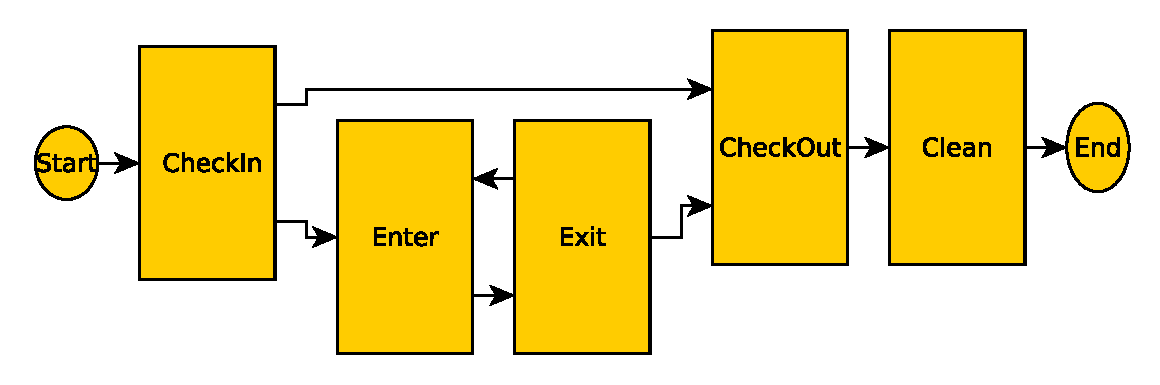
\includegraphics[width=0.9\textwidth]{unnamed0.pdf}
  \end{center}
\end{figure}

\begin{center}

\begin{tabular}{|p{2.5cm}|p{8cm}|}
\hline
\color{blue}{Event} & \color{blue}{Function}\\
\hline
CheckIn & The event that will check a guest who is not currently checked in to the system into a cleaned room that is not current allocated to any other guest.\linebreak This implies a guest can only check-in to one room in the hotel. \\
\hline
CheckOut & This event check a guest out from a room that he/she is allocated to, but not currently occupying. This implies a guest can't check out if he is occupying a room. It also mark the room's clean status to dirty if a guest check out.\\
\hline
Enter & Guest can only enter the room that he is allocated to.\\
\hline
Exit & Guest can exit the room if he is inside the room.\\
\hline
Clean & Clean will always make the room status change from dirty to clean.\\
\hline
\end{tabular}
\end{center}
\section{Design for Refinement}

\subsection{System Conflicts}
\indent The system cannot be refined perfectly by both the original system and the proposed improvement, because the abstract model prevent guest from entering a room that he/she is not checked in to. so that a guest can only enter a room if he is currently checked-in.

However, the original system and the proposed improvement models the authority of guest entering a system be possession of a keycard, this has potentially weaken the guard of the system, because the system assumes that when a guest check out, he/she must lose their possession to the keycard. Otherwise, it is always possible for the previous guest to come back to a room between the period he checks out and the next guest comes in.

However, this happens, because the system assume that if a guest check out, he/she will lose possession of the keycard, which will not necessarily happen in real life.

This security leakage is out side of the system domain, and therefore it can not be fully reflected by the model of the system, therefore K's proposed improvement will not necessarily imply a perfect working system.\\



\subsection{Refinement Strategy}

\noindent\textbf{Task 2: Original System}

\begin{description}
\item [Set of Keys] In the Abstract Model. Keys, card, locks to each room are not present. The state transitions changed from being handled by using a mapping of guest a room to guest to a card that contains two keys, and keys are mapped to room locks.
\item [Partition of Keys] Keys are partition by a set of keys that can be allocated to guest, and a master key, which is exclusively used by cleaners.
\item [Change Keys when a guest first enter a system] Since the system can not distinguish the difference between the first and second key in this model, a extra variable is used called shouldChangeKeys. it is a subset of \verb+{Keys\MasterKey}+.\\if one of the key on the card belongs to should change key and the other doesn't, the system will change the room lock when the guest enter the room, else nothing happens to the room lock when guest enter.\\Also a set of dontAllocKeys is used to ensure the keys will that is not currently used by any rooms will not be allocated since the guest enter this room still has it on his card, this avoid the change of one key card that is able to enter two different room.
\item [Check out] Check out will assure that all keys belongs dontAllocKeys will be restored so it is reusable. This again has to assume that guest lose possession to their card when they check out.
\item [Clean] cleaners can always go to any room since they have a masterkey that is hard coded into the locks.
\end{description}

\noindent\textbf{Task 3: Proposed Improvement}
\begin{description}
\item [Keys] The model contains a set of keys just like the original systems, however since this model of the system requires the ability to distinguish the two keys on the card. The model was change to a mapping of guests to key1 on the keycard named guestCard1, and a mapping to guest to key2 on the card named guestCard2, where the domain of guestCard1 must be the same as guestCard2. This ensure each guest has two distinguishable keys on his card.
\item [Partition of Keys] Keys are partition by a set of keys that can be allocated to guest, and two master keys, which is exclusively used by cleaners.
\item [CheckIn] In this model the cleaner "comes to rescue" so each room is mapped to a cleanerRescued status that is interpreted in the system as a Boolean. Guest can only check into rooms that are rescued by cleaners.
\item [Enter] The model map each rooms door lock to a status called should change or not. If the should change key is TRUE then key store in the room lock will be change from key1 to key2, otherwise not.
\item [Enter without Rescue] Since the guard for enter is changed from allocation of room in the Abstract Model to guest having a key with two distinguishable keys. If the guest check out, and somehow obtained a forged key, he should still be able to go into a room, and this is why the system won't fix the problem and it is out the domain, since the system assume guest lose possession to his/her key when a guest check out a room.
\item[CheckOut] When a guest checks out, the system assume they will lose the key, and set the cleanerRescued status to FALSE, that is a cleaner rescue is required.
\item[RescueCleanMasterKey2] There is an extra event added that is cleaner came to rescue.
\end{description}

\section{Personal comments and Lessons Learnt}

\begin{description}
\item [Event-B] Event-B is a excellent modelling language, it capture the requirements of the system, and by applying set theories and various logic operations it ensure the system to behave with in a certain scope, and a valid set of inputs.
\item [Rodin Platform] Rodin Platform is a good IDE for implementation and model systems in Event-B. It contains three different text editors, and automaticly calculate the proof obligations that is required for the system.\\ Rodin Platform also contains animators, such ProB (the one I use), AnimB, which allows the user to visualise the behavior of the system.\\However there are several bugs experienced with the system.
\color{red}{
\begin{description}
\item [Import \& Export] Since i'm using two different machines, I use the import and export function of rodin a lot, however sometimes this leads to failure of the system.
\begin{description}
\item [animator missing files .bps files are missing]
\item [missing files .bpo files are missing]
\item [imported files missing .bum file]
\end{description}
\item [Solution] import all files again\\ purge all proofs\\ retry auto provers\\ if still doesn't work restart Rodin, and repeat the process
\end{description}
}
\color{black}
\item[Personal Comment] In my first attempt, many proofs could not be automatically performed by the rodin provers, even when I intuitively felt that the events should maintain the invariants that is setted up. However, without modifying the guards for events, I notice that there are two ways to discharge POs.
\begin{enumerate}
\item Use the interactive prover to manually prove the event.
\item Add new unrealistic invariants to machine, or axiom to context to makes the system working. This is legit and valid method such action doesn't change the behavior of events.
\end{enumerate}

\item[FIS Proof Obligation for initialisation] FIS proof obligation undischarged in both original system and proposedimprovement system. That implies that Event-B is uncertain about that system that being modeled is a valid one or not, because initialisating the system by saying every room has a lock wit a key stored in side can be non-achievable if the system doesn't have enough keys.
\item[Future Work, and Comment on System] The system still has flaws after K's improvement, the improvement does not solve the problem. It could be implemented better, if the system ensure that the guest will definitely lose their possession to keys when they check out.
\end{description}



\newpage
\appendix

\section{Reference}
\begin{center}
\textbf{Assignment 1 COMP2111 13s1\\
Cleaners to the Rescue\\}
Kai Engelhardt\\
Revision: 1.3 of Date: 2013/04/09 14:47:11
\end{center}
\end{document}
